\documentclass[11pt]{article}
\usepackage{amsmath}
\usepackage{mathtools}
\usepackage{txfonts}
\usepackage[margin=1.0in]{geometry}
\usepackage{graphicx}
\usepackage{float}
\usepackage{booktabs}
\usepackage[caption=true]{subfig}
\graphicspath{ {images/} }
\usepackage{appendix}
\usepackage{url}
%\usepackage{wrapfig}
\usepackage{algorithm}
\usepackage[noend]{algpseudocode}
\usepackage{caption}


\setlength{\parskip}{\baselineskip}%
\setlength{\parindent}{0pt}%
\renewcommand{\baselinestretch}{1.4}

\title{Regression models for predicting rail transit ridership at the station level}
\author{Daniel Hartig}
\date{\vspace{-5ex}}

\DeclareMathOperator*{\argmin}{arg\,min}


\begin{document}
\maketitle

\section{Introduction}

The United States is undergoing a rail boom. Since 2010, new light rail lines have opened in Dallas, Los Angeles, Salt Lake City, Denver, Minneapolis, Houston, Seattle and more.  A new heavy rail line opened in Washington DC, and a commuter rail system in Orlando. As transit expands in cities in the United States, there is an opportunity to validate predictive rail ridership models. 

A survey of transit agencies \cite{Boyle2006} conducted by the Transit Cooperative Research Program showed that relatively few agencies are using quantitative models when forecasting ridership for new lines, extensions or stations under consideration for funding. Of the 35 agencies that responded to the survey, 29 use professional judgment and 28 use rules of thumb among one or more techniques used to generate ridership forecasts. Another method used by 22 agencies is service elasticity; a set of general transit demand response curves for changing transportation options, published by the Transportation Research Board \cite{tcrp95}. 

For quantitative methods, the most commonly used technique--by 18 of 35 surveyed agencies--is the four-step travel demand model \cite{McNally2008}, introduced by Mannheim and Florian \cite{Mannheim1979, Florian1988}. The Mannheim-Florian model's four steps are trip generation, trip distribution, mode choice and route choice. In the trip generation phase, trip endpoints are created with production and attraction ends. In the trip distribution step, these endpoints are paired up to generate trips; for example a residence is paired with a job location for one trip, or a hotel is paired with a tourist attraction. In the mode choice step, trips are assigned to various transportation modes, such as personal vehicle, bus, or walking. Finally, in the route choice step, a route using that mode of transportation is chosen.

An implementation of the Mannheim-Florian model can be seen in the Seattle's Sound Transit Ridership Forecasting Methodology Report \cite{ST3_2015, ST3_add}. The Sound Transit 3 (ST3) was a ballot measure that passed in 2016 for a \$54 billion expansion of the local light rail system involving 100 km of new tracks and 37 new stations. The ridership forecasting methodology report explained how the project's official ridership projections were developed. The regional area is divided into 785 Alternatives Analysis Zones and for each of these zones transit surveys and recorded ridership on local bus routes were used to complete the trip generation and trip distribution steps. The mode choice and route choice is done using an incremental logit model to predict changes in transit mode based on changes in transit mode availability.

A significant weakness of the four-step method is that it relies on already known transit ridership \cite{NCTR}. For a proposed light rail system, for example, existing bus routes would be used to complete the trip generation and trip distribution steps.

A regression based ridership model could provide an alternative estimate of ridership without depending on previously known transit ridership counts. Only seven of the 35 surveyed agencies used regression models to predict future transit ridership. This thesis proposes a regression-based model using data from the United States Census Bureau at the zip code level. The model will be trained on the zip code characteristics and ridership data from existing light and heavy rail transit systems. The resulting model will be used to predict ridership on other rail transit systems.  

\subsection{Original Contributions}

There are two main objectives of this thesis. The first objective is to investigate the utility of various data from the US Census Bureau as predictor variables in a regression model for urban rail ridership. The second objective is to determine what generalized linear regression methods--in terms of the choice of loss function and link function--are best suited to modeling urban rail ridership given the available data.

This thesis diverges from previous regression modeling by investigating an expanded set of potential features. The US Census Bureau provides extensive data on a per-zip code bases as detailed in Section \ref{sec:data}: there are over a thousand possible features available. This data is provided as counts per zip code. To translate this zip code data into features for a regression model, this thesis presents a novel geographic sampling method in Section \ref{sec:sampling}. 

With features for regression analysis in hand, this thesis benchmarks several different regression methods. Previous regression based analyses of urban rail ridership have exclusively used ordinary least squares regression. This thesis expands the model base to include other loss functions and link functions and reports accuracy metrics for each model. 

\section{Data Sources and Feature Generation}

\subsection{Selection of Transit Systems}

The response variable for the regression analysis is average weekday ridership over a period of at least one year. Ridership data for agencies that publish annual ridership reports is used to validate the model (for ridership data sources, see Appendix \ref{app:ridership}). Six cities were selected for this study: Boston, Chicago, Los Angeles, Atlanta, Dallas, and Denver. Several cities were eliminated from analysis for various reasons. The author was unable to locate ridership information for several cities such as Houston and Miami. A limitation of the Census dataset is that it does not include government employment. While state level employment is significant in all potential cities, state employment levels are relatively constant from city to city. Federal employment varies greatly, however; Washington DC and San Diego with its military installations had to be eliminated due to the large impact of un-recorded federal employment. San Francisco and Philadelphia were eliminated because they have multiple rail systems without integrated fares. New York City was eliminated because its subway has higher ridership than all other intra-urban rail systems in the country combined.

Ridership data is captured by different methods in different cities, but the same underlying data is counted by each case. In Chicago and Boston, the transit agency measures paid station entries. Boston additionally reports transfers between lines at each transfer station. Therefore, daily ridership is measured as the total number of entrances per station per day. This results in one count per one trip; and two counts per one daily commute. Dallas, Denver and Los Angeles report boarding and alighting by train car; so daily ridership is measured as the total number of boardings per stations per day. For transfer stations, boarding is `double counted' since a boarding at station A and a transfer at station B would result in two counts per one trip. Therefore, for these three networks, the transfer stations and their unusually high ridership counts are excluded from the analysis. For Atlanta, the ridership reporting definition is unknown, so we eliminate the one transfer station as a precaution. For Boston and Chicago, ridership is counted by extracting data from the fare system for paid station entries. In Dallas and Denver, passenger counts are measured at the train car by Automated Personnel Counters. In Los Angeles and Atlanta the counting methodology is unknown. 

The data closest to 2015 is used when possible to get an accurate relation between ridership and census data. The census data as well as Chicago, Dallas, and Denver's ridership statistics are from 2015. Boston's ridership is from 2014, Los Angeles' is from 2013-2014, and Atlanta's is from 2010-2013. 

\subsection{Data Sources for Predictor Variables}\label{sec:data}

The zip code level data for feature generation comes from the US Census Bureau and is available at \texttt{factfinder.census.gov}. There over one thousand potential data sets available. We refer to the data available for each zip code as characteristics of the zip code. Selection of features is guided by Kuby \cite{Kuby2004}, Taylor \cite{Taylor2008}, and Currie \cite{Currie2011}, who demonstrate the significance of characteristics such as employment, population, universities, poverty, airports, park and ride stations, and rental housing units. The characteristics can be divided into two categories: counting characteristics and dummy variables. 

This model emphasizes using only features that have `real' units, as opposed to binary features. The only binary dummy variable this model uses as a feature the presence of park-and-ride parking spaces at a transit station. Instead of using measures of land use mix as proposed in other models \cite{Durning2015, Gutierrez2011}, or binary dummy variables for universities and central business districts, the equivalent information is provided naturally as counting data in the feature set. Counts of housing types (such as large apartment buildings versus single family homes) replace land use mix; the number of jobs at universities or in financial jobs provide more information than dummy variables for presence of universities or central business districts. 

\begin{table}[H]
\centering\begingroup\fontsize{10}{10}\selectfont
\begin{tabular}{ll}
\toprule \textbf{Population related}&\textbf{Employment related} \\ 
\midrule Total population&Total Employment pay\\
Population over age 65& Employment in finance industry\\
Population with bachelor's degree& Employment at hospitals\\
Number of residents employed full time&\\
Number of housing units built after 2000&\\
\bottomrule
\end{tabular}\endgroup
\caption{Examples of characteristics associated with zipcodes}\label{tab:char}
\end{table}

The selected characteristics are generally related either to the population of the zip code or the number of jobs of the zip code. The captured characteristics of the built environment, such as the quantity, age, and building type of the housing stock, are generally related to population. For example, the total number of housing units is expected to be highly correlated with the population of a zip code.  Examples of characteristics are provided in Table \ref{tab:char}. Some characteristics, such as total population, are expected to have a positive relationship with ridership; others, such as population under the age of 18, are expected to have a negative relationship. Examples of associations between characteristics and ridership are provided in Figure \ref{fig:chartypes}. A summary of all the selected characteristics is provided in Appendix \ref{app:features}.



\begin{figure}[H]
\centering
\subfloat[An example of a positive association]{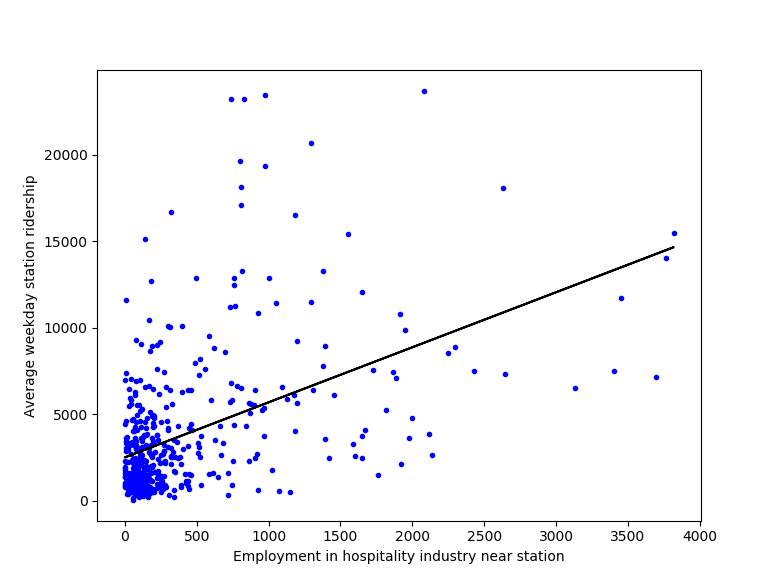
\includegraphics[clip,width=0.5\columnwidth]{exRegPosSlope}}
\subfloat[An example of a negative association]{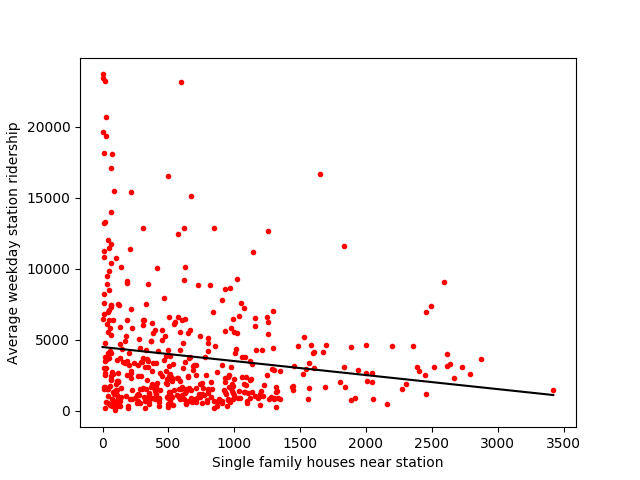
\includegraphics[clip,width=0.5\columnwidth]{exRegNegSlope}}
\caption{Single covariates against the response variable with ordinary least squares (OLS) line of best fit.}\label{fig:chartypes}
\end{figure}


In Yao \cite{Yao2007}, a distinction is made between `Need Index' features, a series of features that depend on the characteristics around the station and are independent of the transit network; and `Transit Network' features, which do depend on the travel time between stations of the transit network. To model network features for each station, the sum of each characteristic for every other station within 15 and 30 minutes transit time is included as a feature of the original station, as described in Section \ref{sec:net}. This provides us a quantitative way to express the 'centrality' dummy variable that is provided as a flag in many models \cite{Kuby2004, Durning2015}. Centrality could be proportional to the count of population or jobs within 30 minutes of a station, for example. 

We translate zip code level data into transit station specific data by sampling each zip code's geographic area to determine proximity to a transit station. For each zip code near the transit network, a set of random points within that zip code is generated using rejection sampling. For each of the those points, one or more closest stations are determined. Each point is assigned to one or more station within walking distance, using the method defined in Section \ref{sec:walk}. Counts for the characteristics of each zip code, such as population or employment, are then assigned to each station proportional to the number of points assigned to each station.

\subsection{Definition of `Walking Distance'}\label{sec:walk}

The area within walking distance of a station is called its `catchment'. To generate a feature for a transit station, the total count of some characteristic within the catchment of that stations is considered. The standard transit catchment distance in literature for rail stations is one half mile (800 m). Guerra \cite{Guerra2012} suggests that one half mile is more appropriate for population as a feature while one quarter mile (400 m) is better for employment as a feature. A case study \cite{ElGeneidy2014} from a 2003 Montreal transit riders origin-destination survey concluded that approximately 50\% of riders of the city's urban rail transit walk less than 500 meters to their stations, while 90\% walk less than 1000 meters. The maximum walking distance is approximately 1500 meters. In another regression-based study of catchment sizes, Gutierrez \cite{Gutierrez2011} found the optimal distance for  for assigning population and employment to a station was between 600 and 900 meters in straight line distance. A straight line distance is measured as the crow flies as opposed to a distance following pedestrian walkways; this distance measurement is consistent with the distances used in this analysis.

A significant concern when tabulating catchments is that in many of the densest regions of cities, there are many stations within a few hundred meters of each other. For example, from the Massachusetts State House in downtown Boston, there are seven urban rail stations on four different train lines within a 10 minute walk, according to Google Maps. Any of those stations could be the `best' place to board and disembark the train for a commute to work at the State House, depending on the direction and train line by which the commuter was arriving in downtown. It is important that we allow some `overlap' in catchment areas; people at one geographic location could use more than one station for various transit needs. 

Given this information, we choose cutoffs of 500 meters and 1000 meters for calculating station distances. For any location that has residents, jobs, or other desired countable characteristics, all stations within 500 meters will be considered equally likely to capture a share of that resident or job's transit demand. If there are no stations within 500 meters; then all stations within 1000 meters will be considered. 

\subsection{Rejection Sampling of Zip Code Shapefiles}\label{sec:sampling}

We translate zip code level data into transit station specific data by using a Monte Carlo method to estimate feature counts near transit stations. Sample points are generated within each zip code near the transit network. Those points are assigned to whichever stations are within walking distance of the station, as defined in Section \ref{sec:walk}. If there are multiple stations within walking distance, then equal fractions of that one point are assigned to each station. The ratio of points assigned to each station to total points generated for each zip code is used to assign feature counts to each station, such that
\[\text{count}(station_i) = \sum_j w_{ij} \cdot \text{count}(zipcode_j)\]
where $w_{ij}$ is the proportion of the points generated in zipcode $j$ that are assigned, wholly or partially, to station $i$. Not all areas within a zip code $j$ will be within walking distance of any station $i$, so 
\[\sum_j w_{ij} \leq 1\] for all $j$. An algorithm for rejection sampling a single zipcode is provided in Algorithm \ref{alg:rejsamp}.


\begin{algorithm}\begingroup\fontsize{10}{10}\selectfont
\begin{algorithmic}
\State{ Given \texttt{zipcode} is a single zipcode near the transit network }
\State{ Let \texttt{zipcode.latrange} and \texttt{zipcode.lonrange} be maximum and minimum latitude or longitude for \texttt{zipcode} shapefile}
\State{ $n\gets$ max(\texttt{zipcode.area} in hectares, 1000)}
\State{ \texttt{randomPoints}$ \gets \{\}$}
\While{ len(\texttt{randompoints}) $< n$}\Comment{Generate \texttt{n} random points within \texttt{zipcode}}
	\State{\texttt{lon }$ \gets $ random number $\in$\texttt{ zipcode.lonrange}; \texttt{lat} $ \gets $ random number $\in$\texttt{ zipcode.latrange}}
	\State {\texttt{point }$ \gets$ (\texttt{lat, lon})}
	\If { \texttt{point} is inside \texttt{zipcode.shapefile} and \texttt{point} is not inside exclusion areas}
		\State{ \texttt{randomPoints }$ \gets$ \texttt{randomPoints }$\bigcup$\texttt{ point}}
	\EndIf
\EndWhile
\For{ \texttt{point} $\in$ \texttt{randomPoints}}\Comment{Assignment of points to stations}
	\State{ $n_{0.5} \gets$ number of stations within 0.5 km of \texttt{point}}
	\State{ $n_1 \gets$ number of stations within 1 km of \texttt{point}}
	\If{ $n_{0.5} > 0$}
		\For{ \texttt{station} within 0.5 km of \texttt{point}}
			\State{\texttt{station.characteristicValue }$  \mathrel{+}= $ \texttt{ zipcode.characteristicValue}$\, / \,n_{0.5}$} 
		\EndFor
	\ElsIf {$n_1 > 0$}
		\For{ \texttt{station} within 1 km of \texttt{point}}
			\State{\texttt{station.characteristicValue }$  \mathrel{+}= $\texttt{ zipcode.characteristicValue}$\, / \,n_1$}	
		\EndFor
	\EndIf
\EndFor
\end{algorithmic}\endgroup\caption{Algorithm for estimating characeristic counts that are near transit stations}\label{alg:rejsamp}
\end{algorithm}



The US Census Bureau provides TIGER/Line shapefiles of each zip code tabulation area (ZCTA) in the United States at \url{https://www.census.gov/geo/maps-data/data/tiger-line.html}. Random points are generated in a rectangular box drawn around the extremities of each zipcode's shape; these random points are accepted if they are within the shapefile or rejected if they are outside it. Those points that are inside the shapefile are tested against author-created exclusion zones. These zones are shapes within the zip code's shapefile area that are known to not have any population, employment, or other countable characteristics. The exclusion zones are mostly drawn over water areas and parks. Those points that are inside the exclusion zones are also rejected. This creates a set of points randomly drawn from the zip code's land area, not counting unoccupied regions like parks. 

The set of points is tested for their distance to any transit stations to determine which station catchments they fall in, as described in Section \ref{sec:walk}. The characteristic counts associated with each tested point are divided between all stations within 500 meters. If there are no stations within 500 meters, then the point is divided between all stations within 1000 meters. If no stations are within 1000 meters, that point is not assigned to any station. The total sum of points and fractional points assigned to each station is divided by the total points available to get the fraction of each of the zip code's characteristic data counts is assigned to that transit station. 

\begin{figure}
\begin{center}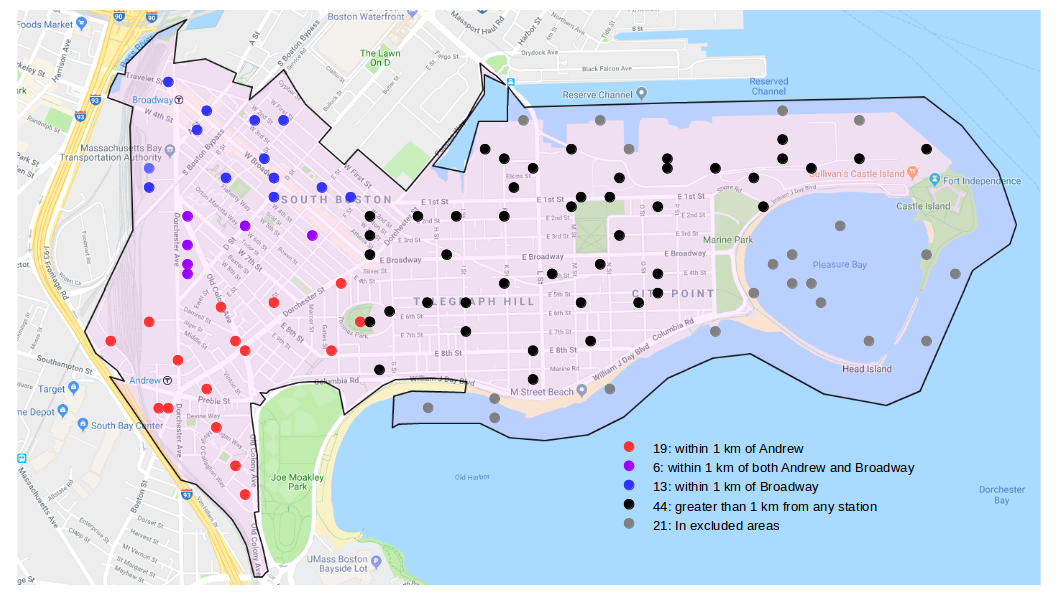
\includegraphics[scale=0.55]{geo_point_demonstration}\end{center}\caption{Illustration of nearest zip code estimation for zip code 02127.}\label{fig:f1}
\end{figure}


An example using zip code 02127, the South Boston neighborhood of Boston, illustrates the sampling method (Figure \ref{fig:f1}). 100 random points are selected within the area of the shapefile. Of these, 21 points indicated in gray are rejected due to exclusion areas based on water area, parks and abandoned port facilities. Of the remaining 79 points, 8 are within 500 meters of Andrew station, while 6 are within 500 meters of Broadway station. Moving out to the 1000 meter radius, 11 are within 1 km of Andrew station, for a total of 19 that are close to Andrew; 7 are within 1 km of Broadway station for a total of 13 that are close to Broadway; and 6 are within 1 km of both. The 6 points within 1 km of both stations are divided evenly between the two. The total population of South Boston is 36494. Therefore, 
\begin{align*}
\text{Counts assigned to station} &= \frac{\text{\# points for one station} \cdot \sum\frac{\text{\# points for multiple stations}}{\text{\# stations for each point}}}{\text{\# points for zipcode}}\cdot\text{characteristic counts}  \\
&= \frac{19 + \frac{6}{2}}{79}\cdot 36494 \text{ people} \\
&= 10163 \text{ people}
\end{align*}
are assigned to Andrew station. Similarly, 7391 people are assigned to Broadway station. Summed over all zip codes near Andrew and Broadway stations, this shows how the total population within walking distance of the station is estimated. This calculation is performed for all countable features and all zip codes and summed total counts for each characteristic are used as a feature for each transit station. 

\subsection{Variance of Monte Carlo estimates}

With any Monte Carlo method for estimation, there is variance in the estimates generated. In this case, the variance comes primarily from the random locations of the points. It is possible that in different Monte Carlo trials, a station may get significantly more or less points nearby it. This is especially significant in areas of high population density; one extra or missing point could be worth hundreds or thousands of jobs in the densest areas of downtown Chicago or Boston. To keep variance to an acceptably low level, we must generate enough sample points that variation between trials is minimal. 

The number of points that will be accepted by rejection sampling is set beforehand. We generate random points, and use rejection sampling to see if they are inside the shape of the zipcode and outside of any exclusion zones. We continue generating points until we have reached the desired number of accepted points.

The land area of the zip codes near the studied transit networks vary in size from as small as 30 hectare in downtown Chicago to as much as 18100 hectares at the suburban end of transit lines in Dallas. To provide an appropriate balance between accuracy and processing speed, we use one accepted point per hectare, but with a minimum limit of 1000 accepted points per zip code. This effectively provides over 10 points per hectare in for the zip codes in the densest parts of the studied networks: the downtown areas of Chicago and Boston. These areas also have the densest network of transit stations, with many stations within a kilometer of each other. In these denser areas, it is important to have enough points that the division of points between stations does not result in too much variance. 

We generate 100 sets of estimates for the a single feature (total population) for all stations in the six transit networks. Figure \ref{fig:mcvar}(a) shows a graph of means of total population estimates against standard deviation of the population estimates, while Figure \ref{fig:mcvar}(b) is means against coefficient of variation. The standard deviation shows an increasing linear relationship with the population mean. The coefficient of variation is never greater than 10.4\% and generally decreases with increasing estimated mean population. The mean coefficient of variance over all studied stations is 5.3\%. By this method, the relative accuracy of any single station estimate of population or employment relative to the mean of 100 estimates of the same feature $\pm$10\% .

\begin{figure}[H]
\centering
\subfloat[Standard deviation versus mean by transit station.]{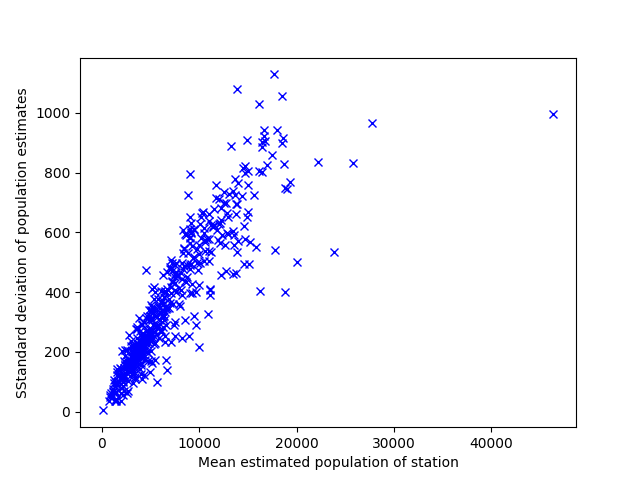
\includegraphics[clip,width=0.5\columnwidth]{estvarstdev}}
\subfloat[Coefficient of variation versus mean by transit station.]{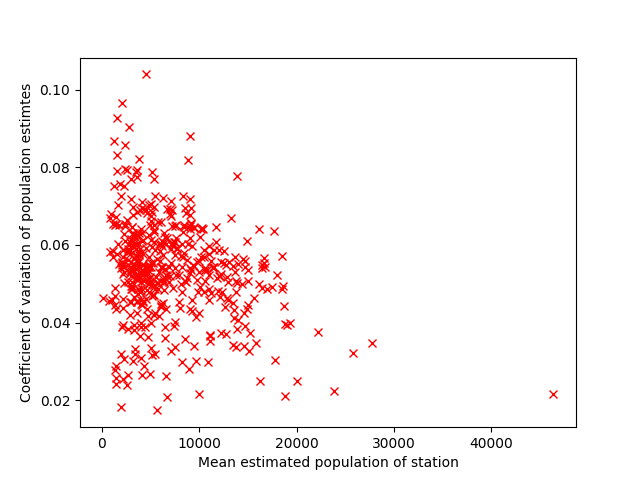
\includegraphics[clip,width=0.5\columnwidth]{estvarcov}}
\caption{Indications of variance for Monte Carlo estimates of the population feature.}\label{fig:mcvar}
\end{figure}

\subsection{Generation of network-dependent features}\label{sec:net}

For each `Need Index' type feature generated by rejection sampling, a set of corresponding network-based features are generated to represent the sum total of a certain characteristic (such as population or employment) within a given travel time of that station. An algorithm for calculating network characteristics is shown in Algorithm \ref{alg:network}. 

\begin{algorithm}
\begin{algorithmic}
\For{\texttt{station}$ \in$ transit network}
	\State\texttt{nearby15} $\gets$ all other stations within 15 minutes travel time of $station$
	\State \texttt{nearby30}$ \gets$ all other stations within 30 minutes travel time of $station$
	\For{every characteristic in the model}
		\For{\texttt{otherStation} $\in$ \texttt{nearby15}}
			\State{\texttt{station.characteristicValue15} $+=$ \texttt{otherStation.characteristicValue}}
		\EndFor
		\For{\texttt{otherStation}$ \in$ \texttt{nearby30}}
			\State{\texttt{station.characteristicValue30} $+=$ \texttt{otherStation.characteristicValue}}
		\EndFor
	\EndFor
\EndFor
\end{algorithmic}\caption{Algorithm for calculating network characteristic counts}\label{alg:network}
\end{algorithm}

The transit network is laid out as a directed graph, where nodes represent the transit stations and edges are weighted by the travel time between the stations. Travel times between stations are available in the transit schedules published by the appropriate transit agencies. Travel times can be different in different directions, following the published schedules. At transfer points, there is a separate node for a single station on each line. The multiple nodes for the same station have edges between them weighted by the average wait time between trains. The wait time is estimated at half the time between trains at the station being transferred to. For example, if one train arrives every 10 minutes, then a transfer to a node on that line at any station will have an estimated travel time of 5 minutes. Many transit agencies align arrival times so that one line will depart a few minutes after another train arrives. No attempt is made to capture this more complicated arrangement of estimated transfer times. 

\begin{figure}
\begin{center}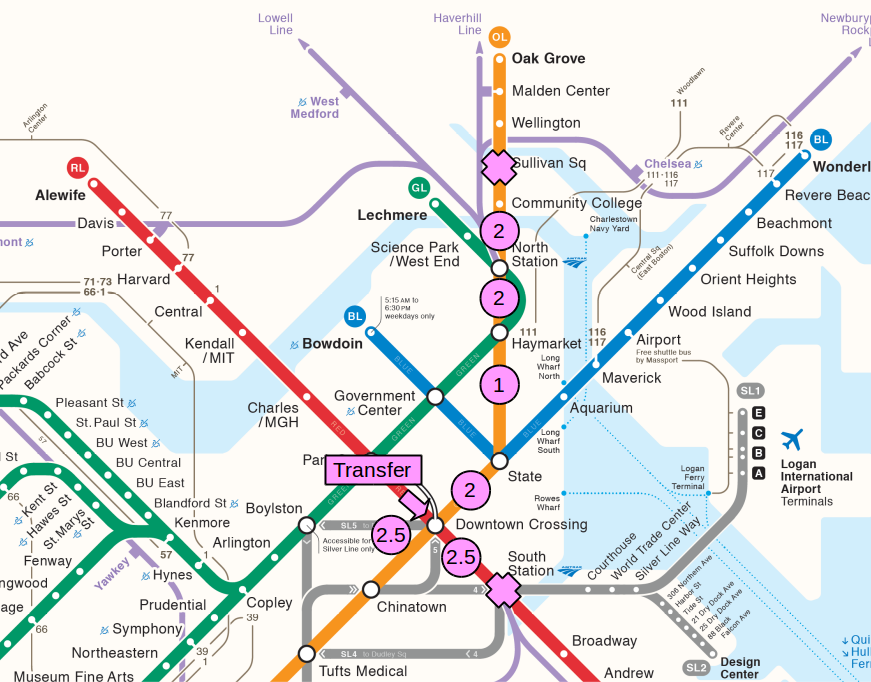
\includegraphics[scale=0.7]{transfer_demonstration}\end{center}\caption{Illustration of travel time calculation for Sullivan Square to South Station, in Boston.}\label{fig:f2}
\end{figure}

An illustration of the calculation of travel time between Sullivan Square and South Station in Boston is provided in Figure \ref{fig:f2}. Starting at Sullivan Square on the Orange Line southbound, there are four edge traversals totaling seven minutes to get to Downtown Crossing. From there, there is a 2.5 minute wait until a Red Line (also Southbound) train arrives, and 2.5 more minutes of travel to South Station. The total travel time is thus twelve minutes. 

For any given station, we find a set of all stations within aX distance by selecting an ego graph out of the entire transit network. An ego graph is a sub-graph containing all nodes that are within a specified distance of the central node. 

For each station $A$ and for the set of all stations ($S$) within 15 minutes of $A$; the counts of each `Need Index' type feature is summed over all stations of $S$. This is the count used for the corresponding network type feature of $A$. The same procedure is repeated for all stations within 30 minutes of $A$. Thus, for each `Need Index' type feature associated with a station in the feature set, there are two additional features: one summing the counts of that feature within 15 minutes and one within 30 minutes.

These features are important for providing a measure of centrality to the network. Stations near the center of the network and at transfer points between lines will have higher counts of network features than peripheral stations. The other important function of the network features is to provide estimates of the total scale of system ridership. The more people, jobs, and other characteristics near transit stations, the higher the overall system ridership is expected to be. This is a key component of the model's portability between different city's transit networks. 

\subsection{Analysis of zip code characteristics by city}
%\vspace{-15pt}
\begin{figure}
\centering
\subfloat[Boston - Blue; Chicago - Red; Los Angeles - Green]
{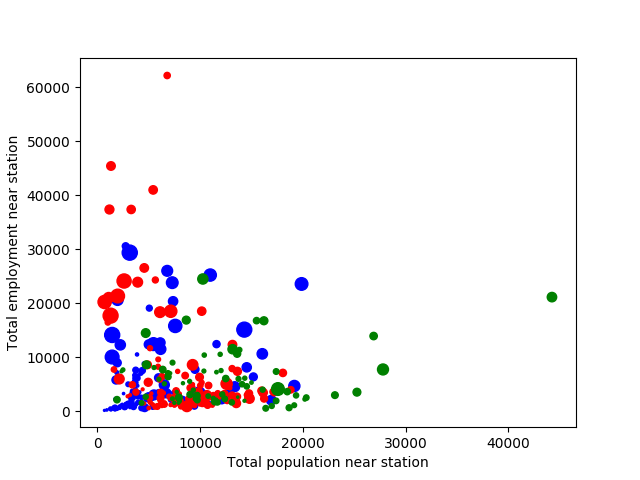
\includegraphics[clip,width=0.8\columnwidth]{localvars_large}}

\vspace{-15pt}
\subfloat[Atlanta - Blue; Dallas - Red; Denver - Green]{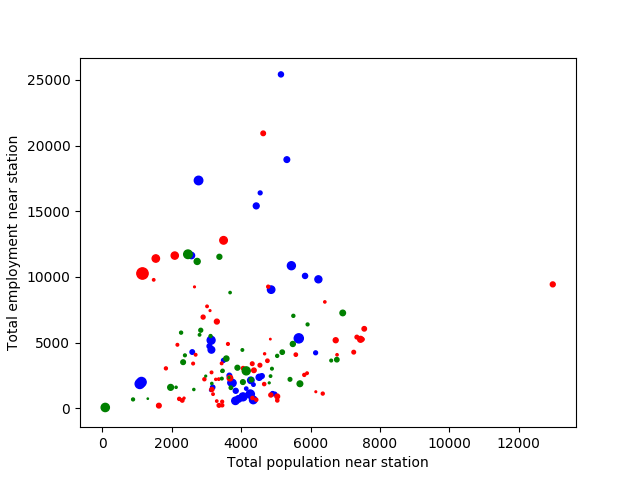
\includegraphics[clip,width=0.8\columnwidth]{localvars_small}}
\captionsetup{singlelinecheck=off, justification=centering}
\caption[]{Employment against population with a 15 minute transit ride for sets of three transit networks.\linebreak
Area of marker represents ridership of the station}\label{fig:localvars}
\end{figure}

The purpose of including multiple transit networks with varying levels of ridership is to ensure that the model captures a broad range of relationships between employment, population and other zip code characteristics on the one hand, and transit ridership on the other. Figure \ref{fig:localvars} shows the employment and ridership counts within walking distance assigned to each station on the transit networks. The ridership of each stations is proportional to the area of the marker for each station. We can see that there is a wide range of population and employment figures near transit stations. In our selection of six transit networks, some networks have much higher peaks of certain zip code characteristics than others, so the graphic is divided into two subfigures, one for the higher ridership networks and one for the lower. 

Station remoteness has a significant impact on the characteristics of stations. For example, the five highest population transit stations are all in Los Angeles. It is not true that the densest areas of Los Angeles have a higher population density than Boston or Chicago. Rather, the Los Angeles transit network has lower station density than Boston or Chicago in the areas of highest population density. Therefore, some stations in high population density areas of Los Angeles will have a transit catchment of up to two square kilometers. For Boston or Chicago, with closer station spacing and multiple lines, any point in the areas of highest population density will have four or more stations within walking distance.  

\begin{table}
\centering\begingroup\fontsize{10}{10}\selectfont
\begin{tabular}{l|cccc}
\toprule Network City&Total Population&Total Employment&Network length (km)&Avg Weekday Ridership \\ 
\midrule Chicago&1189454&872206&157&608472\\
Boston&622484&656375&98&591823\\
Los Angeles&935041&436846&169&254183\\
Atlanta&150171&207601&77&150237\\
Dallas&255092&261813&150&96069\\
Denver&161542&170631&149&75128\\
\bottomrule
\end{tabular}\endgroup
\caption{Network wide characteristics for the six transit networks considered in this thesis}\label{tab:netsize}
\end{table}

The overall characteristics of each transit network are found in Table \ref{tab:netsize}. There is a positive linear relationship between both population and employment and ridership at the network-wide level. However, the effect of network length is also significant. For example, Atlanta's population and employment near its transit stations are both lower than that of Dallas, but Atlanta's ridership is fifty percent larger. Atlanta's network length is about half that of Dallas, suggesting that Atlanta's transit accessible population and employment are compressed into a much smaller area. This density appears to be a significant factor in Atlanta's higher ridership. However, looking at Figure \ref{fig:localvars}(b), where Atlanta's stations are in the blue and Dallas' in red, it is not clear that Atlanta's stations have any individual advantage in population and employment. 

This shows the necessity of the network-dependent features. In Figure \ref{fig:networkvars}, we see the sum of population and employment within a 15 minute transit rider of each station, instead of within walking distance of each station. In Figure \ref{fig:networkvars}(b) we see that Atlanta's smaller network and more tightly spaced stations means that stations generally have more other stations within a given travel distance. Therefore, many of Atlanta's stations have higher network population and employment counts than their corresponding stations in Dallas. The inclusion of the network features will allow the regression model to more accurately predict the higher ridership for stations in Atlanta. 


\begin{figure}
\centering
\subfloat[Boston - Blue; Chicago - Red; Los Angeles - Green]
{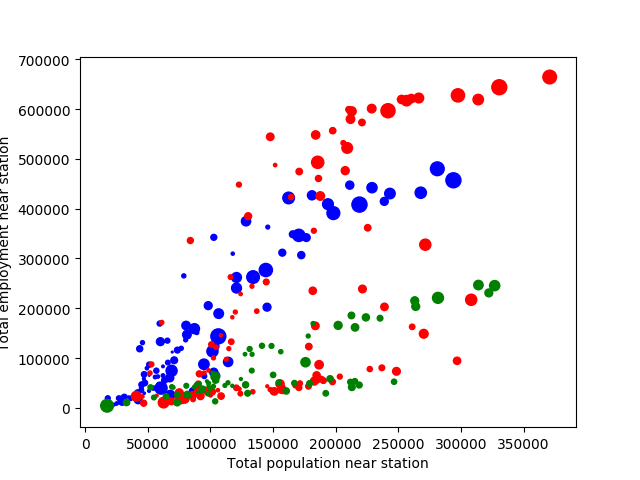
\includegraphics[clip,width=0.8\columnwidth]{networkvars_large}}

\vspace{-15pt}
\subfloat[Atlanta - Blue; Dallas - Red; Denver - Green]{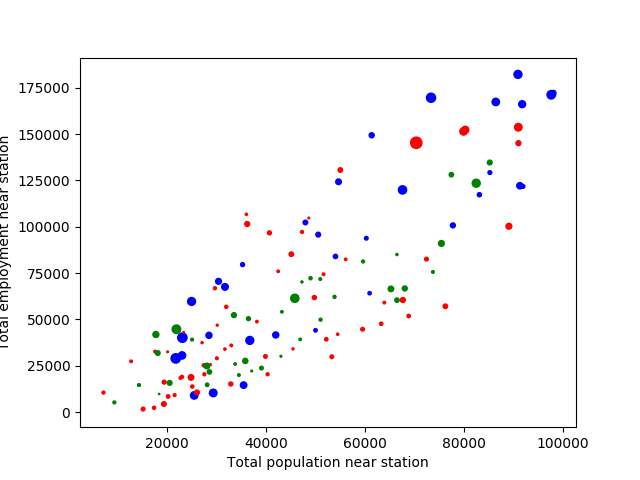
\includegraphics[clip,width=0.8\columnwidth]{networkvars_small}}
\captionsetup{singlelinecheck=off, justification=centering}
\caption[]{Employment against population with walking distance for sets of three transit networks.\linebreak
Area of marker represents ridership of the station.}\label{fig:networkvars}
\end{figure}

\pagebreak
\begin{appendices}

\section{Data sources}

\subsection{Ridership data}\label{app:ridership}
\begingroup
\fontsize{9}{10}\selectfont
\begin{tabular}{ll}
Los Angeles: & \url{http://libraryarchives.metro.net/DPGTL/Ridership/RailActivityByStationFY2014.xls} \\
Chicago:& \url{http://www.transitchicago.com/assets/1/ridership_reports/2015_Annual.pdf} \\
Atlanta:& \url{http://documents.atlantaregional.com/transportation/TFB_2014_v17.pdf}\\
Boston:& \url{http://archives.lib.state.ma.us/bitstream/handle/2452/266319/ocm18709282-2014.pdf} \\
Denver:& \url{http://www.rtd-denver.com/documents/serviced/lrt-activity-08-2015.pdf} and \\
& \url{http://www.rtd-denver.com/documents/serviced/lrt-activity-Jan-April-2016.pdf}\\
Dallas:& \url{https://www.dart.org/about/dartreferencebookmar16.pdf}\\
\end{tabular}
\endgroup

\subsection{US Census feature data sources}\label{app:features}

All feature data is accessed through the American Factfinder website at \url{factfinder.census.gov}.

\begingroup
\fontsize{9}{9}\selectfont
\begin{tabular}{ll}
Population&Table DP05, Item HC01\_VC03\\
Population, 18 and under&Table DP05, Item HC01\_VC03 - Item HC01\_VC32\\
Population, 65 and over&Table DP05, Item HC01\_VC37\\
Housholds&Table S1101, Item HC01\_EST\_VC02\\
Households with Children&Table S1101, Item HC01\_EST\_VC06\\
Families&Table S1101, Item HC01\_EST\_VC010\\
Population with at least Bachelors degree&Table S1701, Item HC01\_EST\_VC34\\
Population in labor force&Table S1701, Item HC01\_EST\_VC37\\
Employed population&Table S1701, Item HC01\_EST\_VC38\\
Full-time employed population&Table S1701, Item HC01\_EST\_VC47\\
Population living at greater than 500\% of poverty level&Table S1701, Item HC01\_EST\_VC56\\
Population living at less than 200\% of poverty level&Table S1701, Item HC01\_EST\_VC01 -  HC01\_EST\_VC59\\
Housing units&Table DP04, Item HC01\_VC03\\
Single-family detached housing units&Table DP04, Item HC01\_VC14\\
Housing units in duplexes or townhouses&Table DP04, Items HC01\_VC15 + HC01\_VC16\\
Housing units in structures of 3-9&Table DP04, Item HC01\_VC17 + HC01\_VC18\\
Housing units in structures of 10+&Table DP04, Item HC01\_VC19 + HC01\_VC20\\
Housing units built before 1940&Table DP04, Item HC01\_VC36\\
Housing units built after 2000&Table DP04, Item HC01\_VC27 + HC01\_VC28 + HC01\_VC29\\
Housing units occupied by owner&Table DP04, Item HC01\_VC65\\
Housing units occupied by renter&Table DP66\\
Number of Jobs&Table CB1500CZ11, Item ‘EMP’\\
Total pay of all jobs&Table CB1500CZ11, Item ‘PAYANN’\\
Number of jobs at hospitals&Table CB1500CZ21, NAICS code 622, Estimated\\
Number of jobs at universities&Table CB1500CZ21, NAICS code 6113, Estimated\\
Number of jobs in hospitalitiy field&Table CB1500CZ21, NAICS code 72, Estimated\\
Number of jobs in finance field&Table CB1500CZ21, NAICS code 52, Estimated\\
Number of jobs in professional fields&Table CB1500CZ21, NAICS code 54, Estimated\\
Number of jobs in entertainment fields&Table CB1500CZ21, NAICS code 71, Estimated\\
\end{tabular}
\endgroup

\end{appendices}

\bibliographystyle{unsrt}
\pagebreak\bibliography{bibrefs}

\end{document}